%% LyX 2.3.4.2 created this file.  For more info, see http://www.lyx.org/.
%% Do not edit unless you really know what you are doing.
\documentclass[english]{article}
\usepackage[latin9]{inputenc}
\usepackage{amsmath}
\usepackage{amssymb}
\usepackage{graphicx}
\usepackage{babel}
\begin{document}
\title{Model O}
\maketitle

\section*{Model of Delta}

Weekly cases $X_{t},$ simple model

\begin{equation}
X_{t}=r_{t}I_{t-1}c_{t-2}s_{t-1}X_{t-1}+\epsilon_{t}\label{eq:main}
\end{equation}
where $r_{t}$ is the ``basic reproduction number'' (see later),
$c_{t}$ is the contact reduction ($1$ corresponds to pre-pandemics),
$s_{t}=1+\gamma\cos(at+b)$ where $\gamma(=0.18)$ is a constant and
$a,b,$ are such that the period is one year and the max is in the
half of January, $\epsilon_{t},\text{\ensuremath{\mathbb{E}\epsilon_{t}=0} }$is
a residuum with standard deviation $\sim X_{t-1}$ and 
\begin{equation}
I_{t}=(1-\frac{u_{t}}{\alpha})V_{t},\qquad V_{t}=(1-v_{t}-w_{t})\label{eq:i}
\end{equation}
is the immunity coefficient where $\alpha(=0.4)$ is the ascertainment,
\[
u_{t}=(\rho\circ x)_{t},\qquad w_{t}=(\psi\circ b)_{t}
\]
where $\rho$ is the waning of natural immunity ($=2\%$ a month),
$\psi$ is the booster waning (probably same as second dose waning),
$x_{t}=\frac{\sum_{s}^{t}X_{s}}{population},$ $b_{t}=\frac{B_{t}}{population}$,
$B_{t}$ is the number of boosters and $\circ$ is convolution. With
full (1 or 2 shot) vaccination it is a bit more complex. 
\[
v_{t}=(\phi\circ f^{t})_{t}
\]
where $\phi$ is the immunity waning of final doses (=5\% a month),
$f_{\tau}^{t}=\frac{F_{\tau}^{t}}{population}$, $F_{\tau}^{t}$ is
the number of people who got final doses at $\tau$ but did not get
boosters by $t$. 

Practically
\begin{itemize}
\item $r_{t}$ can be estimated by regression (since July 21 should be constant
$r_{t}=r^{\delta}$), 
\[
\frac{X_{t}}{X_{t-1}}=r^{\delta}\underbrace{I_{t-1}c_{t-2}s_{t-1}}_{\text{independet var}}
\]
\item $X$ (hence $x$) can be got from public datasets
\item $F$ and $B$ probably best from ockovani.csv (boosters can be got
as difference total-first-second)
\end{itemize}
Note: when computing the model, it may happen due to a rough time
interval that $I_{t}<0$. Thus, we have to adjust its computation
as 
\[
I_{t}=[1-\frac{u_{t}}{\alpha}]^{+}V_{t}.
\]


\section*{Omicron}

Denote $Y_{t}^{v}$ the numbers of omicron infections given that previous
infection by infection delta did not take place and $Y_{t}^{\delta}$
the number of those who had delta before. Assume that $Y_{\tau}^{v}=i$
for some (import) $i$ and starting time $\tau$ and $Y_{\tau}^{\delta}=0,Y_{t}^{v}=0,Y_{t}^{\delta}=0,\tau<t.$
Put $Y_{t}=Y_{t}^{\delta}+Y_{t}^{v}.$ Let (\ref{eq:main}) keep holding
with $r_{t}=r^{\delta}$ and
\[
u_{t}=u_{t}^{\delta},\qquad u_{t}^{\delta}=(\rho\circ y^{v})_{t}+(\rho\circ(x-y^{\delta}))_{t}+(\rho\circ y^{\delta})_{t}=(\rho\circ(x+y^{v}))_{t}
\]
where$y_{t}^{v}=\frac{\sum_{s}^{t}Y_{s}^{v}}{population}$, $y_{t}^{\delta}=\frac{\sum_{s}^{t}Y_{s}^{\delta}}{population}$. 

As for Omicron, we assume, for $t>\tau$,
\[
Y_{t}=r^{o}J_{t-1}c_{t-2}s_{t-1}Y_{t-1}+\varepsilon_{t}
\]

where
\[
J_{t}=\left[1-\frac{e\times(\rho\circ(x-y^{d}))_{t}+y_{t}^{d}+(\rho\circ y^{v})_{t}}{\alpha}\right]^{+},\qquad W_{t}=1-(\iota v_{t}+\upsilon w_{t}),\qquad
\]
where $\iota,\upsilon\in[0,1]$ is the omicron's immunity escape from
finished vaccination, booster, respectively, immunity (one means no
escape). Note that we assume 100 per cent immunity after double infection.
However, this does not disinguish reinfections (after delta) and new
infections. To get this, observe that the population fraction not
having reported infection is $u^{ov}=x_{t}+y_{t}^{v}$ so the virgin
population is $1-\frac{u_{t}^{ov}}{\alpha},$ hence

\[
Y_{t}^{v}=r^{o}J_{t-1}^{v}c_{t-2}s_{t-1}Y_{t-1}+\varepsilon_{t},\qquad J_{t}^{v}=\left[1-\frac{u_{t}^{ov}}{\alpha}\right]^{+}W_{t};
\]
Consequently, 
\[
Y_{t}^{d}=r^{o}J_{t-1}^{d}c_{t-2}s_{t-1}Y_{t-1}+\varepsilon_{t},\qquad J_{t}^{d}=J_{t}-J_{t}^{v}
\]


\section*{Estimation of $\alpha$}

From regression
\begin{multline*}
\frac{X_{t}}{X_{t-1}}=r^{\delta}(1-\frac{u_{t}}{\alpha})(1-v_{t}-w_{t})c_{t-2}s_{t-1}\\
=r^{\delta}\underbrace{(1-v_{t}-w_{t})c_{t-2}s_{t-1}}_{1st\text{independet var}}+\underbrace{\beta}_{=-\frac{r^{\delta}}{\alpha}}\underbrace{u_{t}(1-v_{t}-w_{t})c_{t-2}s_{t-1}}_{\text{2nd independent var}}
\end{multline*}


\section*{Hospitalization}

Data show that number $H_{t}$ of newly admitted to hospital best
correlate with $X_{t}$, These are data from autumn 2021 (boxes):

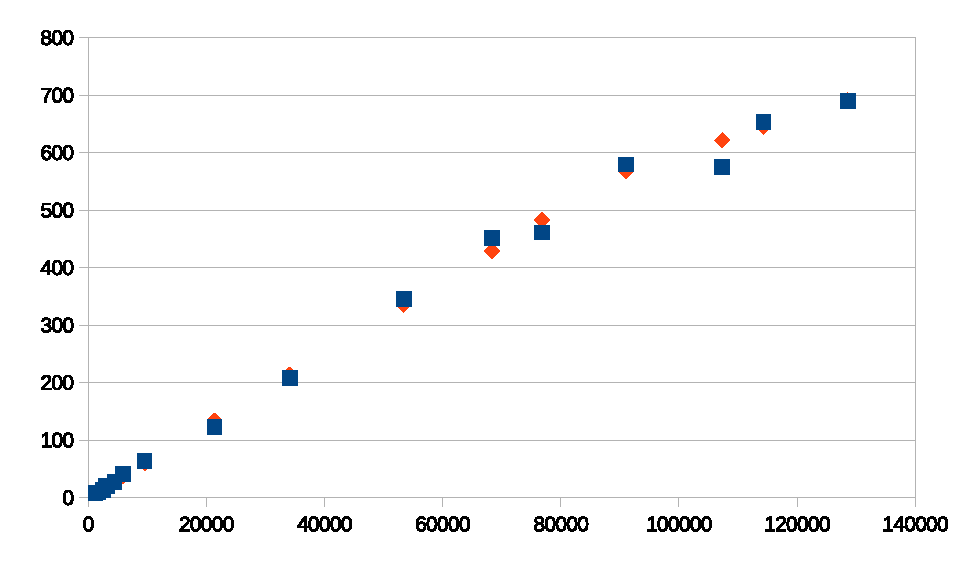
\includegraphics[scale=0.8,bb = 0 0 200 100, draft, type=eps]{../../ModelO/h.eps}

The graph shows a nearly perfect linear dependece up to approx 550
admissions, then there is a kink. We fit this as 

\[
H_{t}=f(\gamma^{\delta}X_{t})\qquad f(x)=x-\delta(x-\eta)^{+},\qquad\gamma^{\delta}=0.00628,\delta=0.4802,\eta=565
\]
(diamonds show the fit). 

With $o$ variant present, we will assume 
\[
H_{t}=f(\gamma^{\delta}X_{t}+\gamma^{o}Y_{t})
\]
 for some $\gamma^{o}$.

\section*{Simulation of Omicron onset}

As a base, we take waning parameters from {[}Andrews et al., Effectiveness
of COVID-19 vaccines against the Omicron (B.1.1.529) variant of concern,
https://www.medrxiv.org/content/10.1101/2021.12.14.21267615v1.{]}:
$\iota=0.5,\upsilon=0.8.$ We assume that the reduction $e$ of post-infection
immunity is similar to that of boosters. Further we, in line with
Report 50 of Ferguson et al. (https://www.imperial.ac.uk/media/imperial-college/medicine/mrc-gida/2021-12-22-COVID19-Report-50.pdf?fbclid=IwAR2OB0rvk9l7N4dFR6YlN84Od-4\_hAWzXKPC-UrWe1pPpzSp2E6eqcgICeA)
assume that the hospitalization rate of omicron is approx two times
less than that of delta. According to accumulating evidence, we estimate
$r^{o}$ to be around 2.5 times more than $r^{\delta.}.$\footnote{The growth rate $r^{o}$ can a\r{u}sp be computed from the reported
doubling time $d$ by formula 
\begin{equation}
r^{o}=\exp\{7\ln(2)/d\}/J,\qquad J=(1-eu)(1-(\iota v+\upsilon w))=(1-e\times0.5)(1-(\iota\times0.3+\upsilon\times0.3))\label{eq:rom}
\end{equation}
Here, $J$ is the omicron's immunity factor in UK at time of omicron
onset. (after imposing into the omicron's regression equation, it
produces the weekly grow corresponding to the doubling time $d$). }Further, by the latest estimate by UZIS, omicron now forms about one
tenth of cases, which means that $i\doteq5000$ by December 27.

We compute $3^{5}$ scenarios by perturbing following parameters
\begin{itemize}
\item $\iota\in\{0.4,0.5,0.6\}$
\item $\upsilon\in\{0.7,0.8,0.9\}$
\item $e\in\{0.7,0.8,0.9\}$
\item $r^{o}\in\{2r^{\delta},2.5r^{\delta},3r^{\delta}\}$ 
\item $\gamma^{o}\in\{0.4\gamma^{\delta},0.5\gamma^{\delta},0.6\gamma^{\delta}\}$ 
\end{itemize}

\end{document}
